\section{Evaluation}\label{sec:evaluation}
\todo[inline]{Might need to rerun the benchmarks on a better machine, as Roulette is too slow right now. Also want to add in bit blast to the results, currently it's way too slow to execute on my machine.}

This section confirms that the performance of \Slice{} is competitive with existing state-of-the-art exact and approximate inference solvers for hybrid probabilistic programs. In particular, we evaluate \Slice{} using Dice and Roulette backends against the exact inference solver SPPL~\cite{Saad2021SPPL} and the approximate inference solver HyBit~\cite{Garg2024BitBlast} on various benchmarks. Our evaluation consists of three sets of programs. First is a series of synthetic benchmarks designed to test the how well \Slice{} scales asymptotically compared to SPPL. Second is a set of benchmarks for verifying fairness properties of decision trees. Lastly, we evaluate \Slice{} on a series of small baseline programs commonly used to test PPLs in the literature. 

\subsection{Experimental Setup}\label{sec:experimenal-setup}
All experiments were run on a ..., using the original version of Dice (2020) from Holtzen et. al.~\cite{Holtzen2020Dice} and the most recent version of Roulette that relies on Racket 8.13 and Rosette 4.1. Each experiment was carried out using a consistent-effort approach, with the goal of determining the most effective encoding for the program in each language and making sure that programs were equivalent across all languages. 

\subsection{Synthetic benchmarks}\label{sec:synthetic-benchmarks}
To evaluate the asymptotic performance of \Slice{}, we designed seven synthetic benchmarks that stress-test different variants of probabilistic programs with continuous distributions. Currently, there are no benchmarks in the literature that test scaling of continuous programs, and we seek to close this gap. Each benchmark generates programs that grow linearly in size in the number of comparison tests (e.g. number of $<$ operators) to measure how execution time scales. This bears resemblence to how scalability is tested for discrete PPLs in the litearture: by growing the program by adding one additional layer to the chain of \texttt{flips} that depends on the previous. Doing so results in a path enumeration that grows exponentially in the number of layers. We generate programs of varying structure:

\subsubsection{Conditional Independence.} 
If a variable \texttt{z} is conditionally independent of \texttt{x} given \texttt{y}, then \texttt{y} acts as a kind of interface between \texttt{x} and \texttt{z} that allows inference to be split into two separate analyses. Bayesian networks use conditional independence to compactly represent complex distributions, for example. We test programs where each variable's distribution depends on comparisons with previous variables, specifically when:

\begin{itemize}
\item Each variable depends on its immediate predecessor variable through conditional statements. This creates a chain of dependencies where $x_i$ depends on whether $x_{i-1} < c$ for some constant $c$. See Figure~\ref{fig:cond-benchmarks-a}.
\item Each variable depends on a randomly chosen predecessor variable through conditional statements. This creates a chain of dependencies where $x_i$ depends on whether $x_1, ..., x_{i-1}$ chosen uniformly at random is $< c$ for some constant $c$, but note this could lead to unused variables. See Figures~\ref{fig:cond-benchmarks-b} and~\ref{fig:cond-benchmarks-c}, where the former guarantees unique distributions for each variable whereas the latter generates random ones.
\end{itemize}

\begin{figure}[!t]
\centering
\begin{subfigure}{0.32\textwidth}
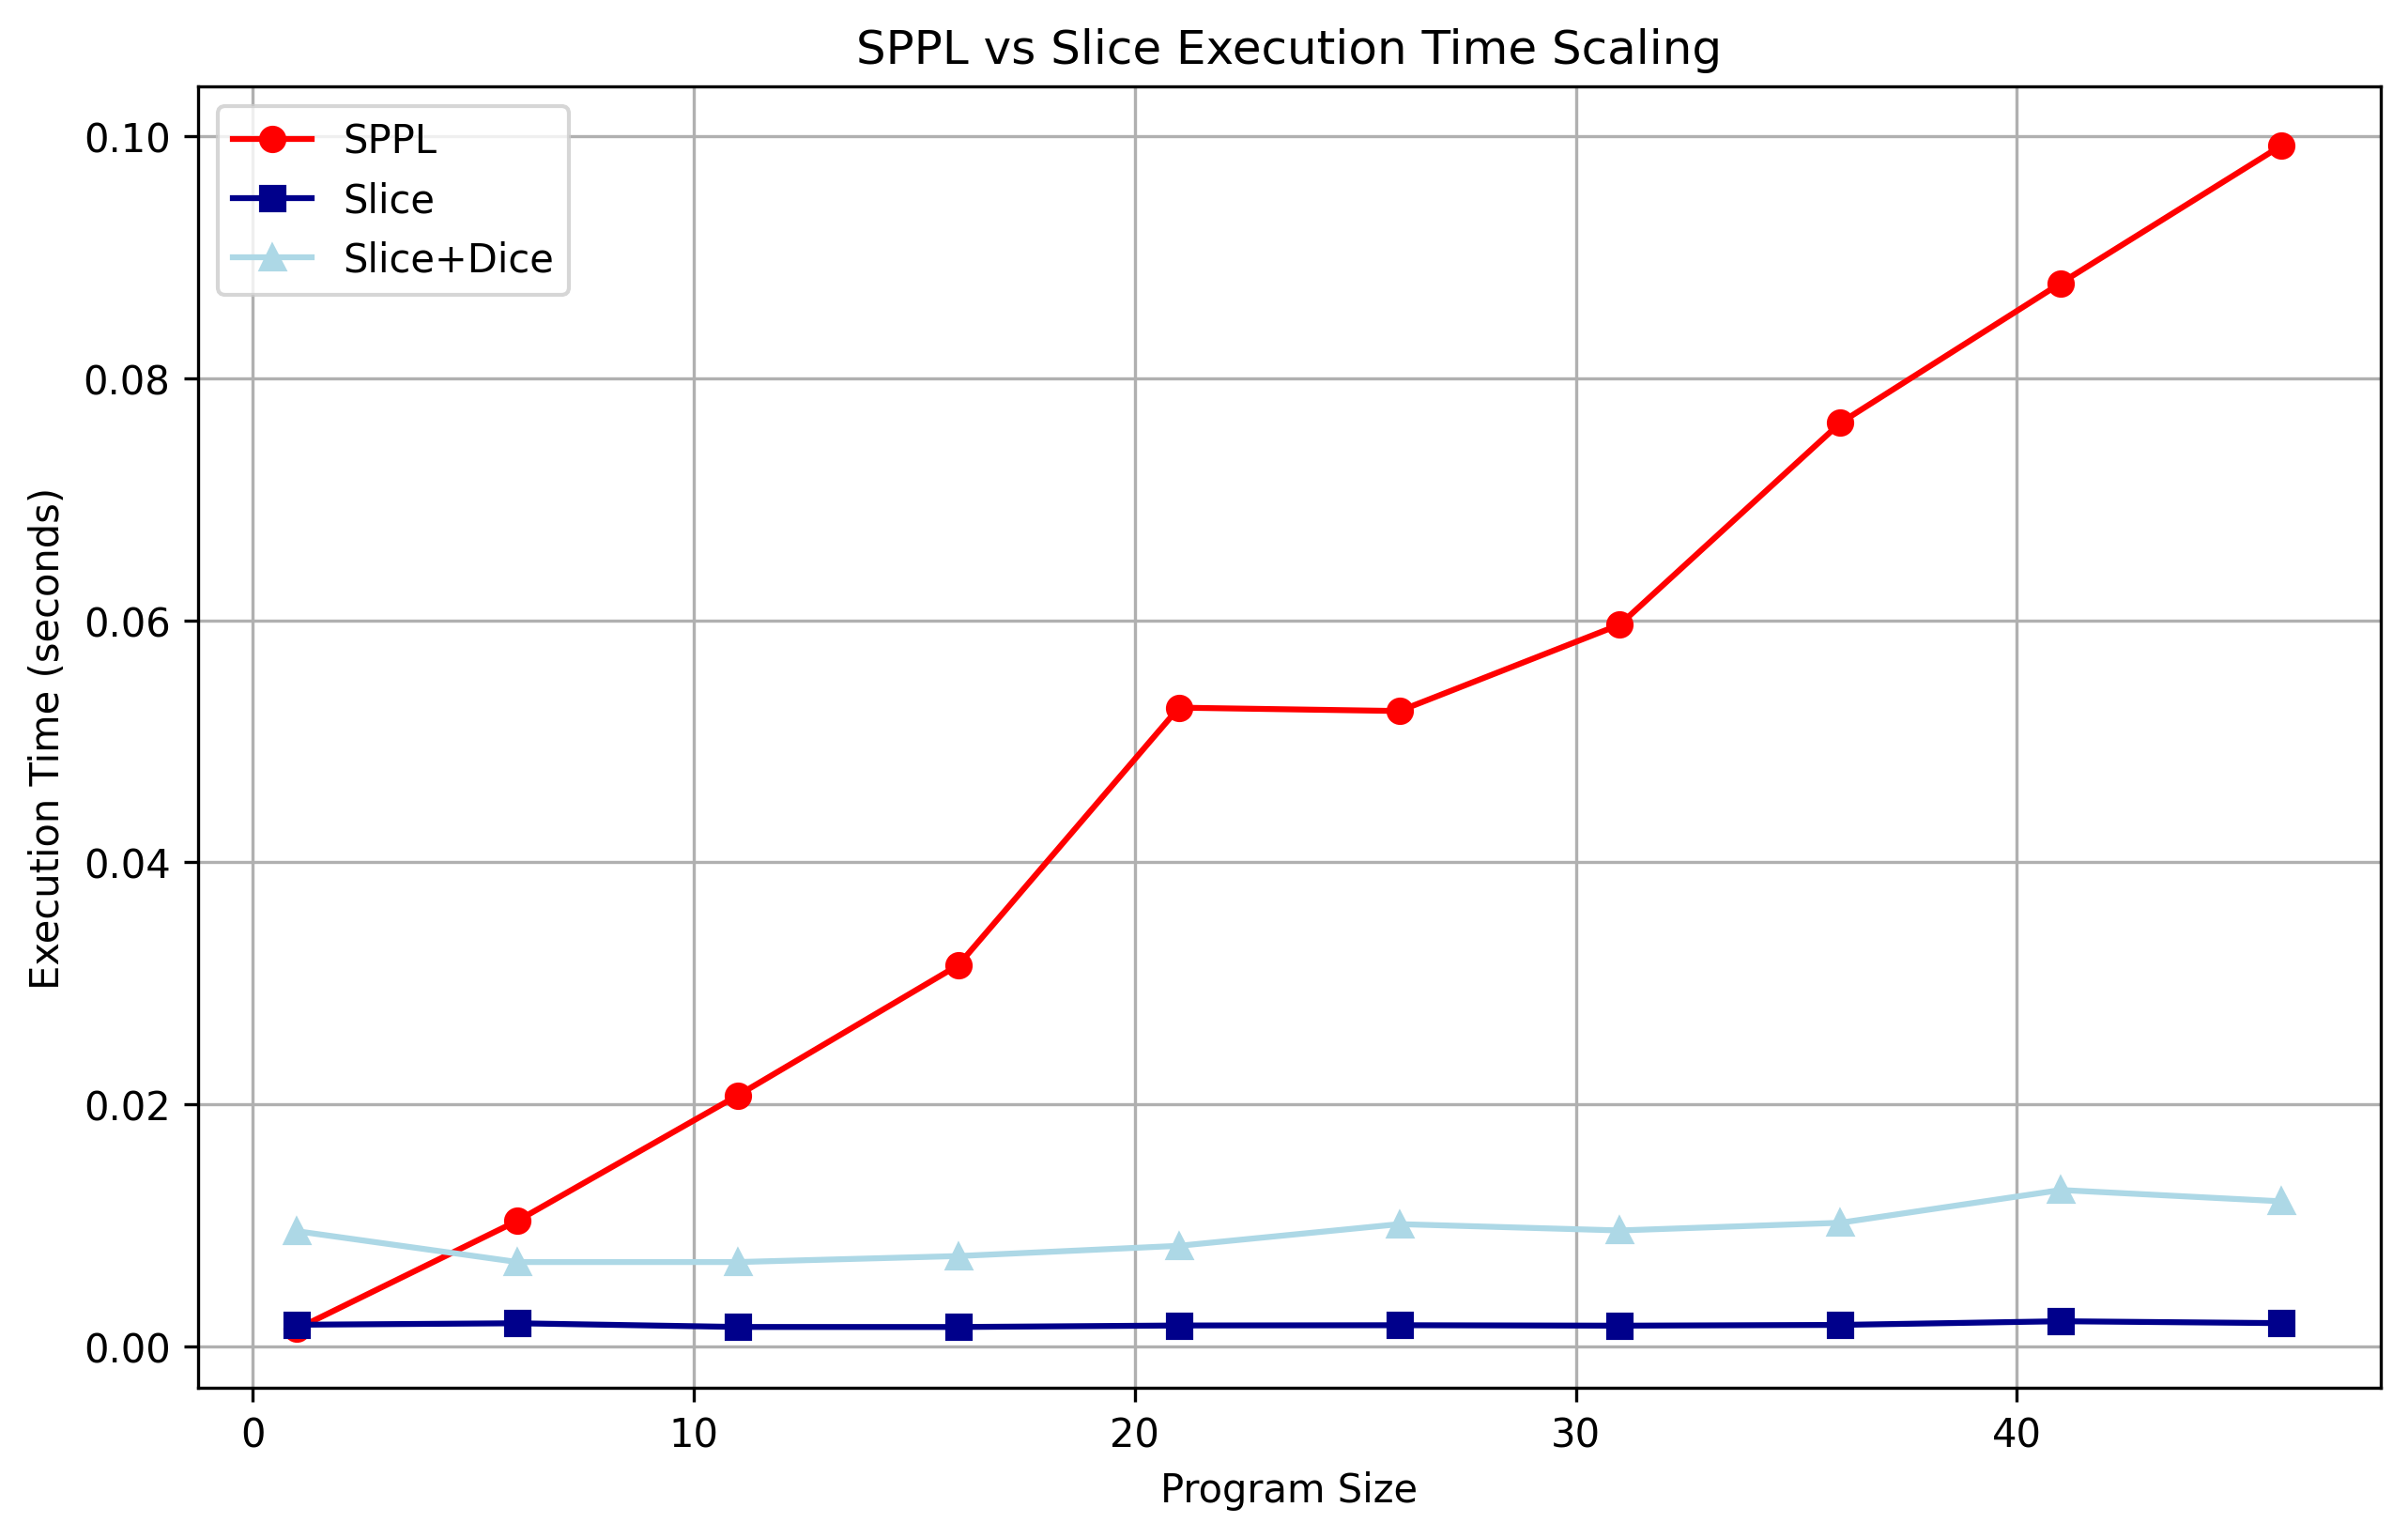
\includegraphics[width=\textwidth]{../images/scaling/build_conditional_independent_slice.png}
\caption{Conditional Independent}
\label{fig:cond-benchmarks-a}
\end{subfigure}
\hfill
\begin{subfigure}{0.32\textwidth}
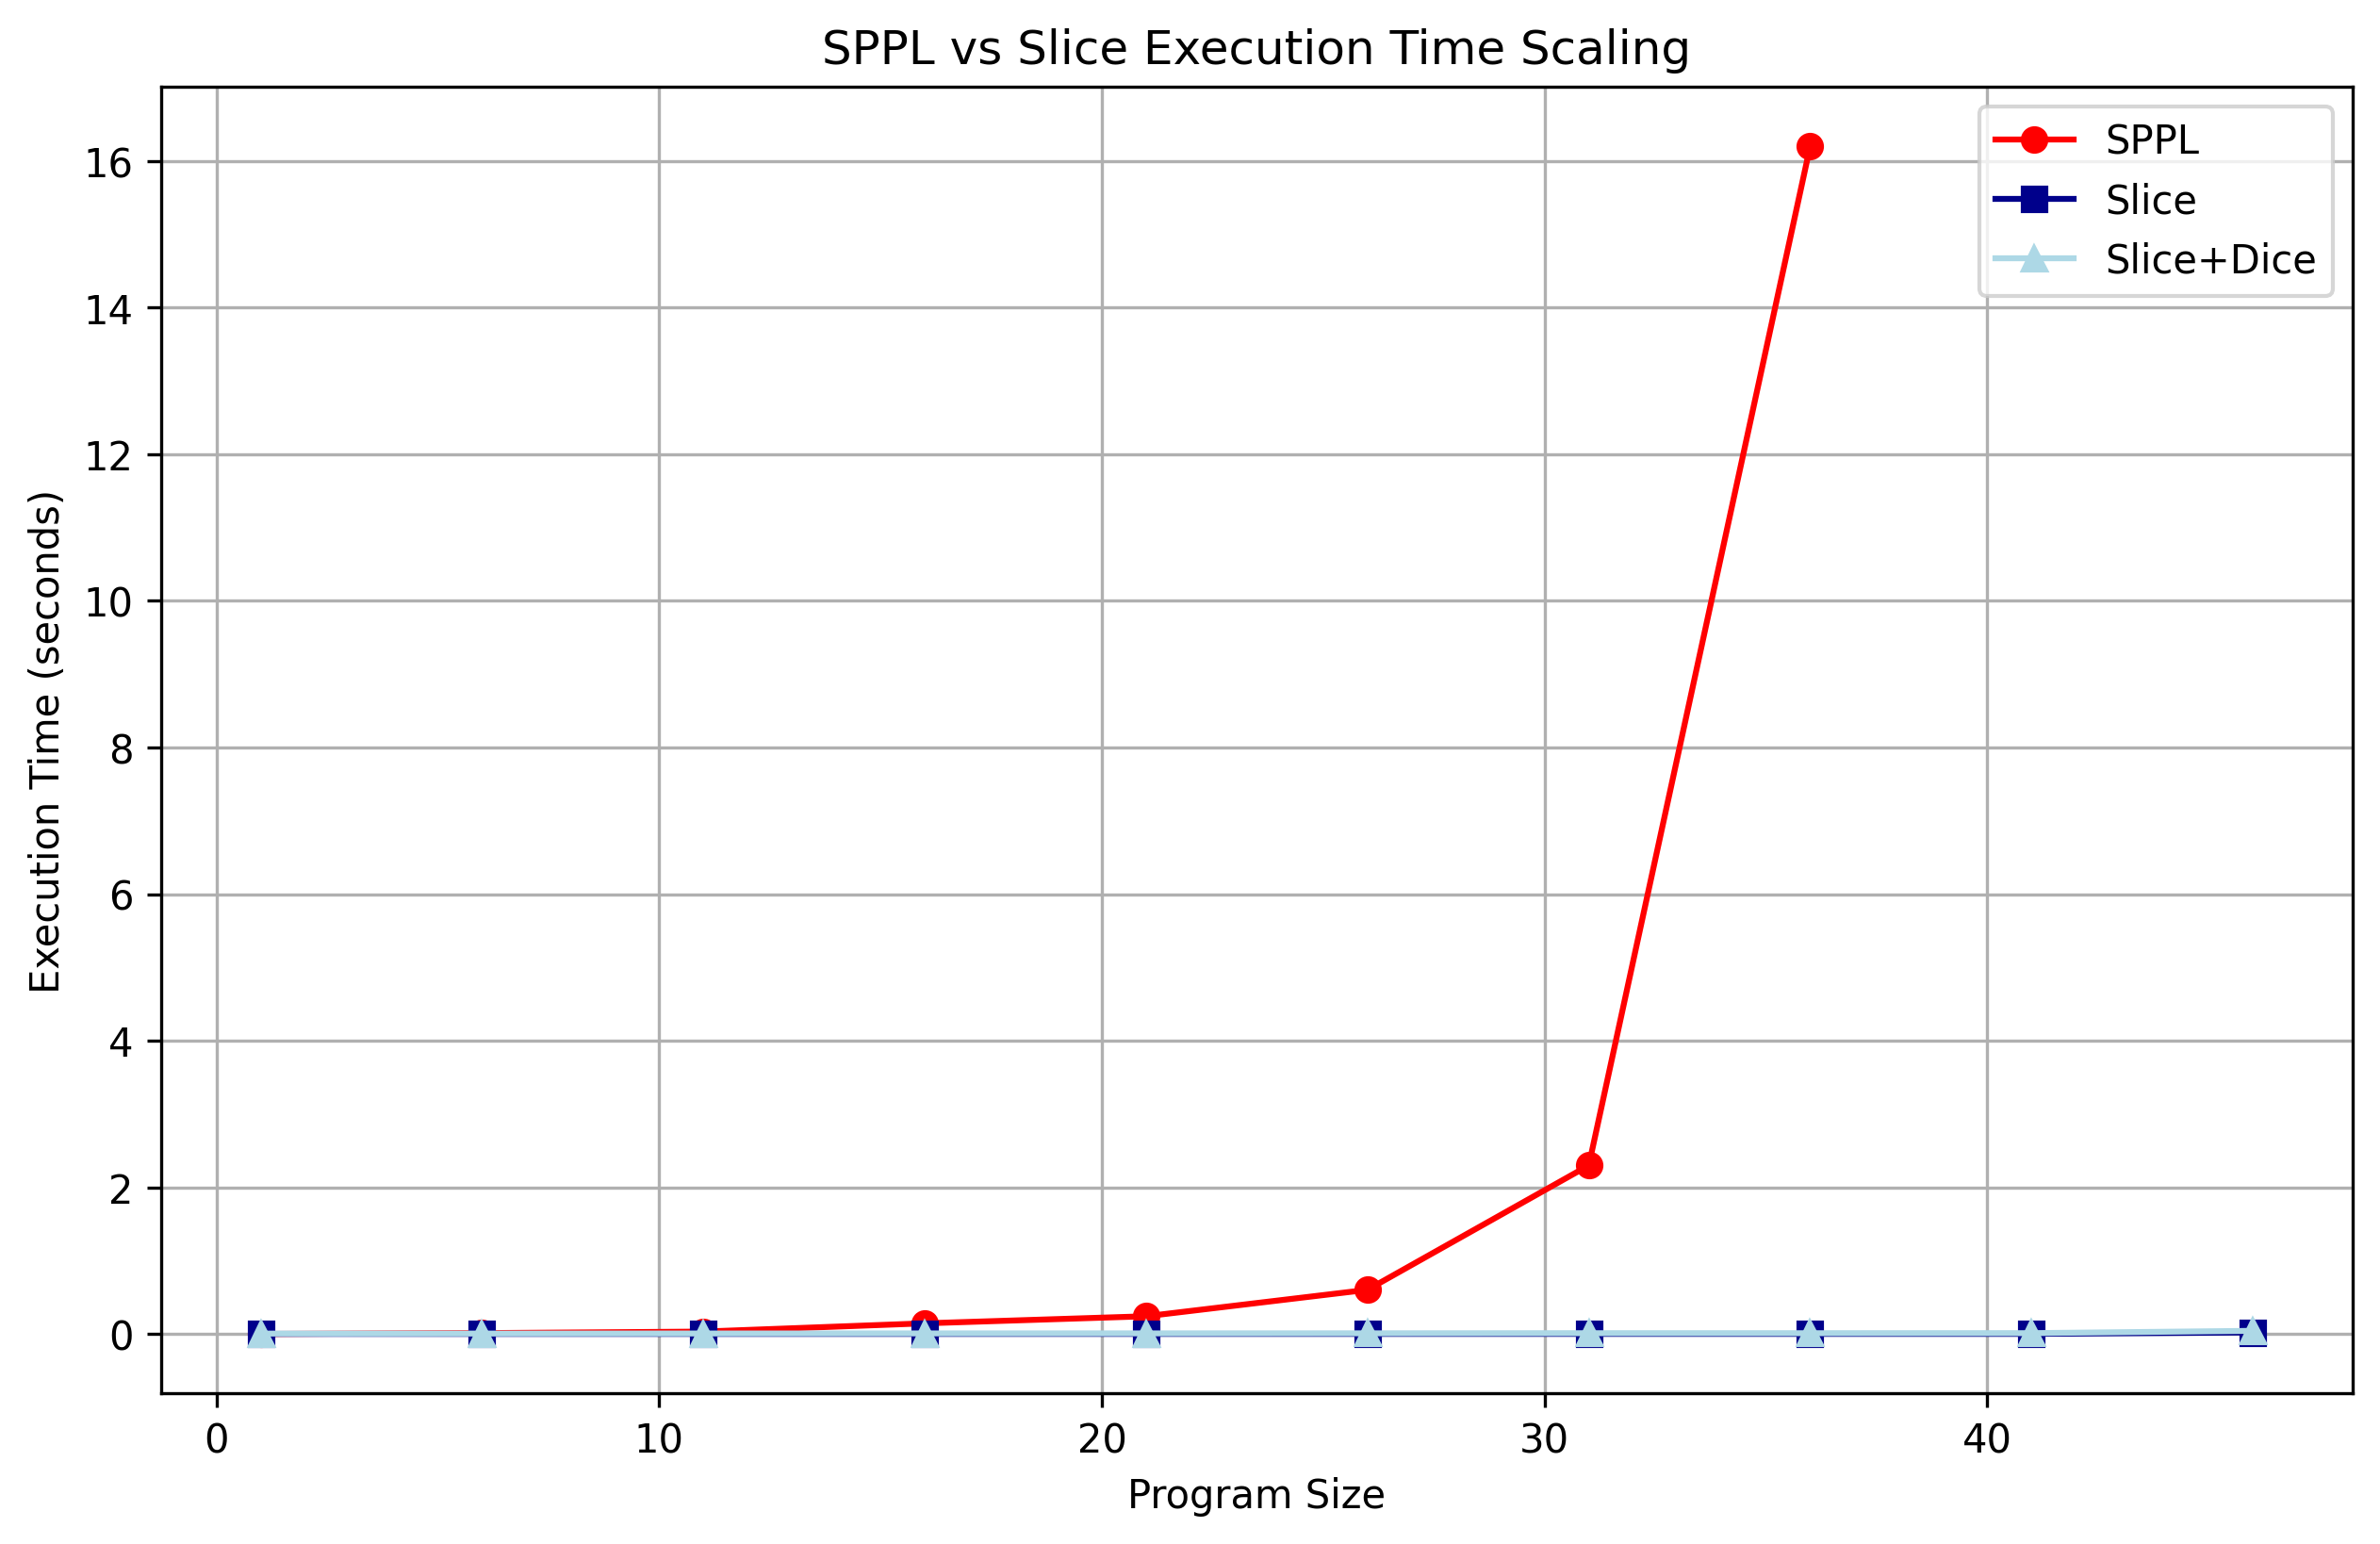
\includegraphics[width=\textwidth]{../images/scaling/build_conditional_random_independent_slice_1.png}
\caption{Conditional Random 1}
\label{fig:cond-benchmarks-b}
\end{subfigure}
\hfill
\begin{subfigure}{0.32\textwidth}
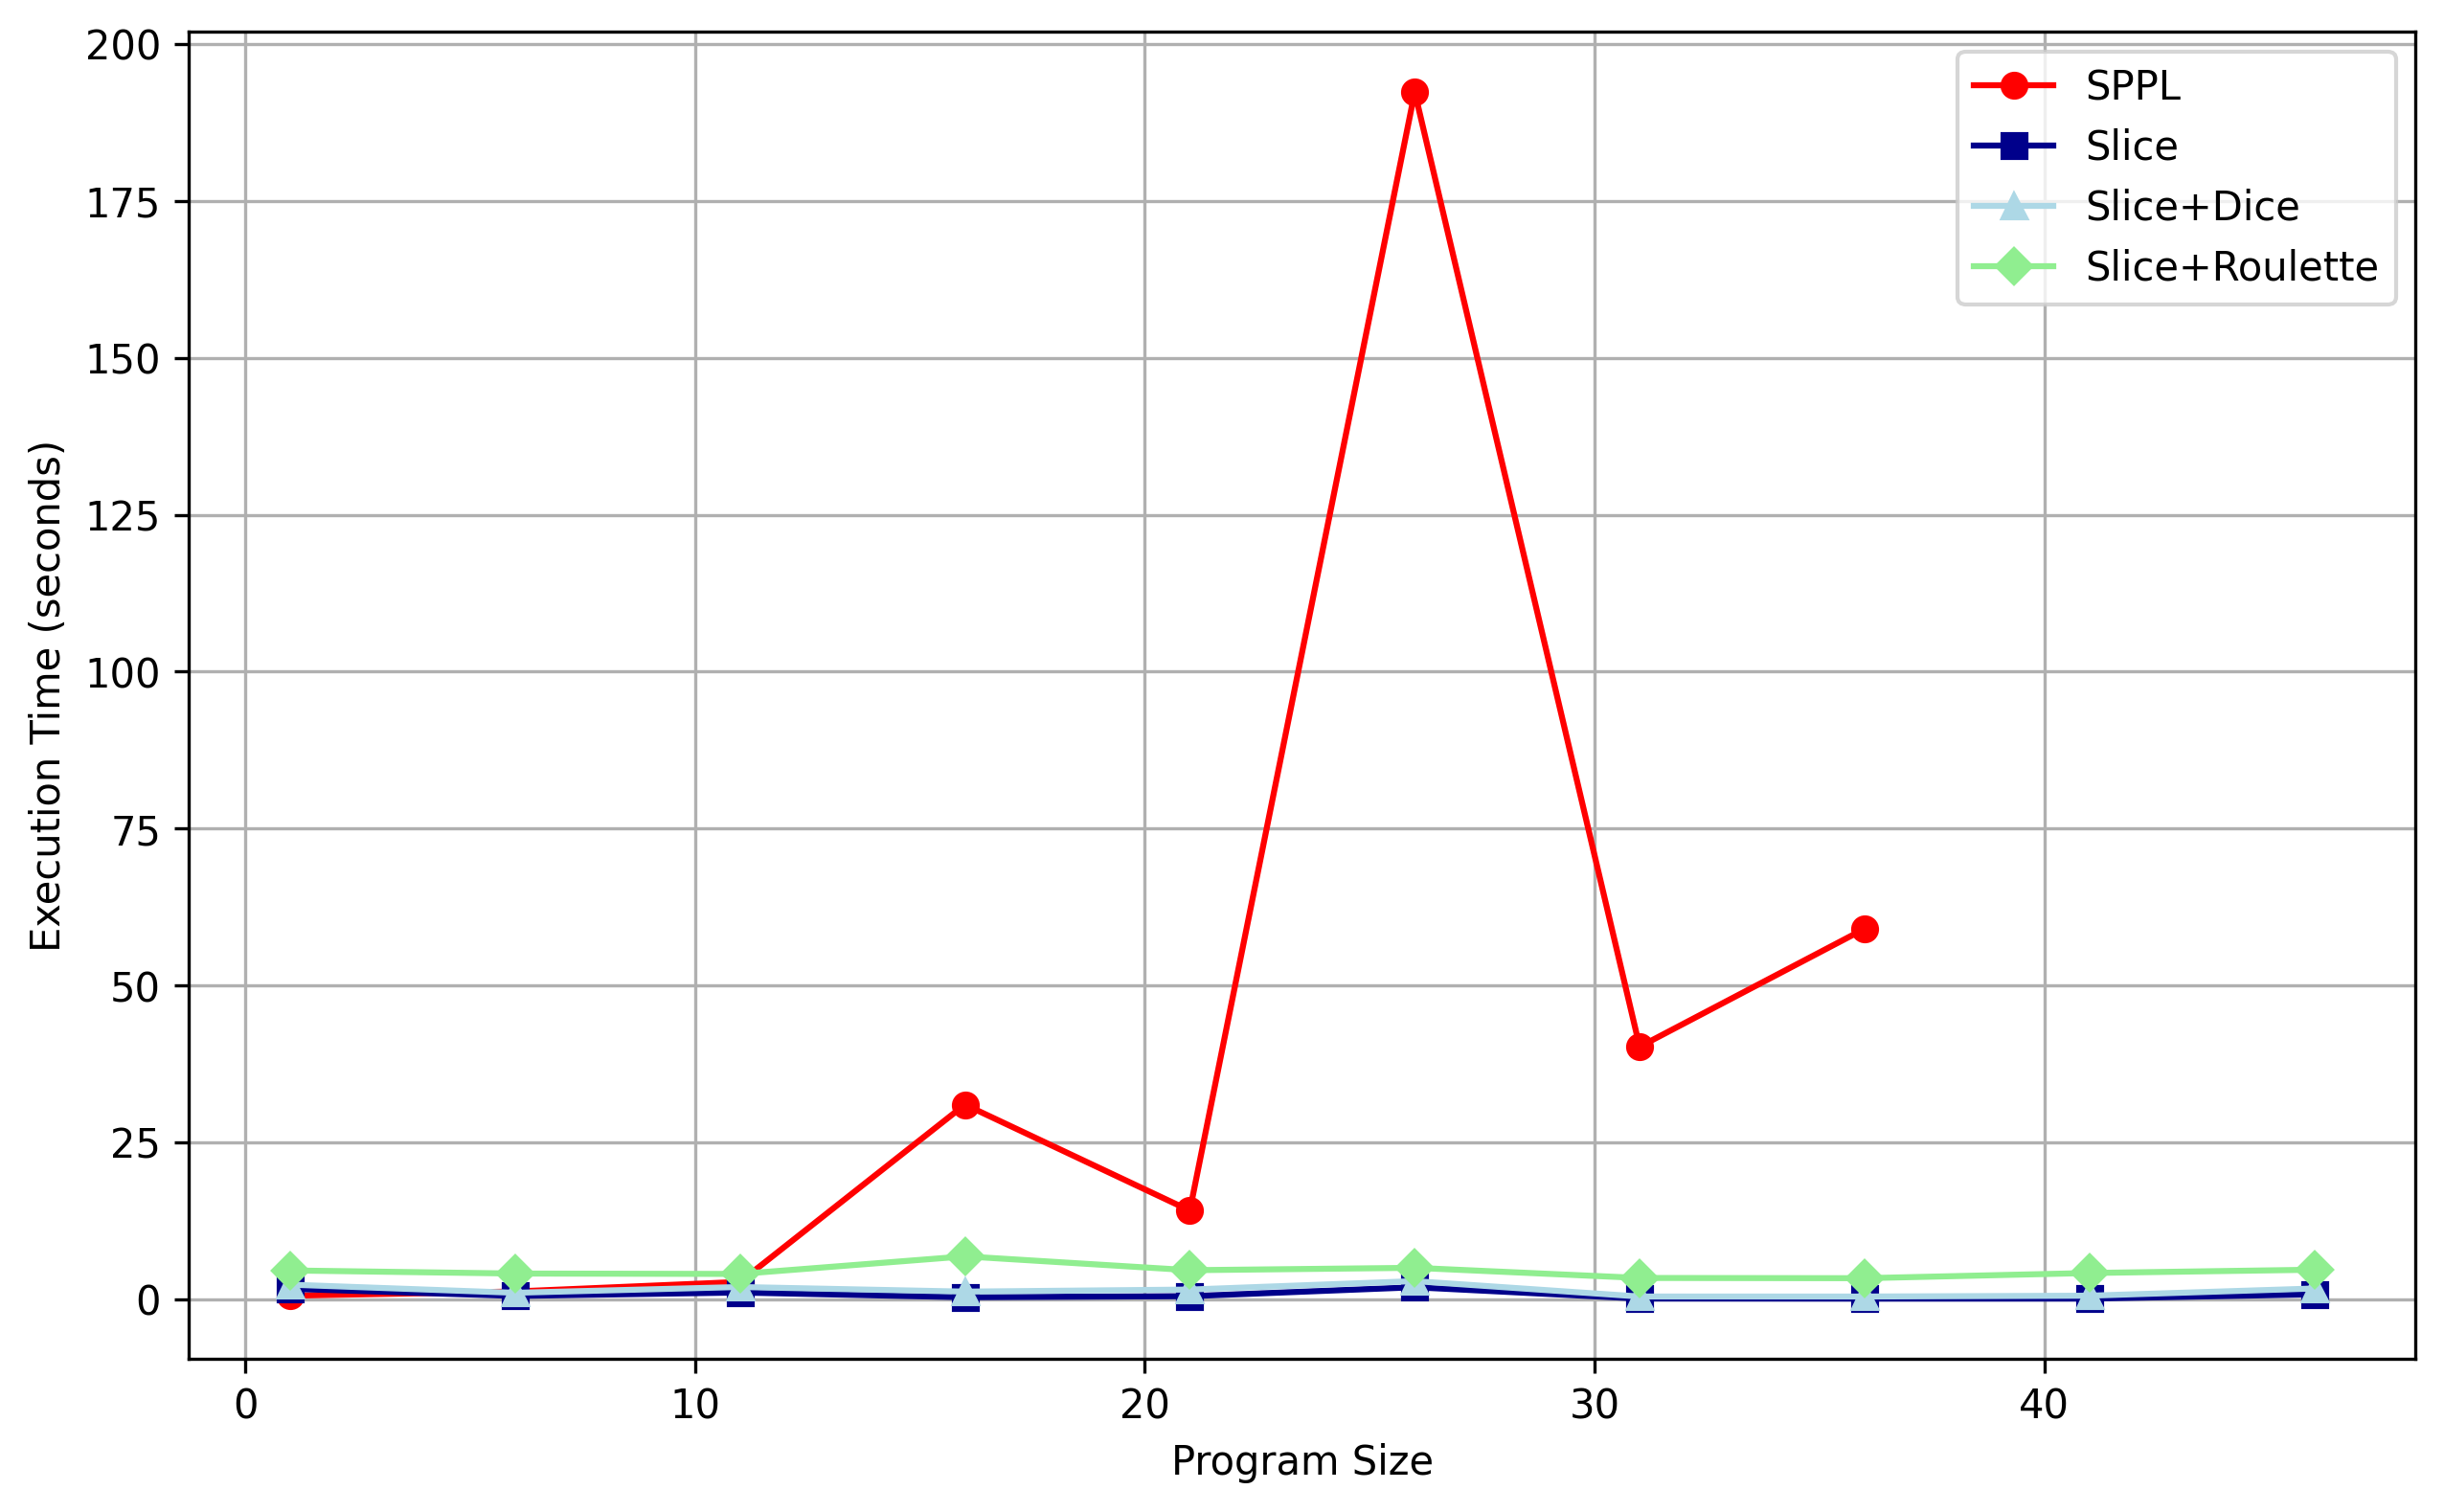
\includegraphics[width=\textwidth]{../images/scaling/build_conditional_random_independent_slice_2.png}
\caption{Conditional Random 2}
\label{fig:cond-benchmarks-c}
\end{subfigure}
\caption{Scaling results for conditional independence benchmarks. SPPL (red) shows exponential growth and times out early, while Slice (blue), Slice+Dice (light blue), and Slice+Roulette (light green) maintain near-linear scaling.}
\label{fig:cond-benchmarks}
\end{figure}

\subsubsection{Alternating Guards.}
We test programs with alternating comparison patterns,
where the control flow depends on earlier random variables. This pattern is characteristic of hierarchical or history-dependent probabilistic programs. Specifically, we test when:

\begin{itemize}
\item Variables in conditionals alternate based on a guard span parameter. For example, with span 3, guards cycle through $x_1, x_2, x_3, x_1, x_2, x_3, ...$ See Figure~\ref{fig:alt-benchmarks-a}. Since such programs may have unused variables, we remedy this by generating programs whose if-else bodies depend on the immediate predecessor variable; see Figures~\ref{fig:alt-benchmarks-b} and~\ref{fig:alt-benchmarks-c}.

\item Variables in conditionals alternate based on a guard span parameter, but we randomly choose the guard span parameter in each iteration instead of it being deterministically chosen as before. See Figure~\ref{fig:alt-benchmarks-d}.
\end{itemize}

\begin{figure}[!t]
\centering
\begin{subfigure}{0.48\textwidth}
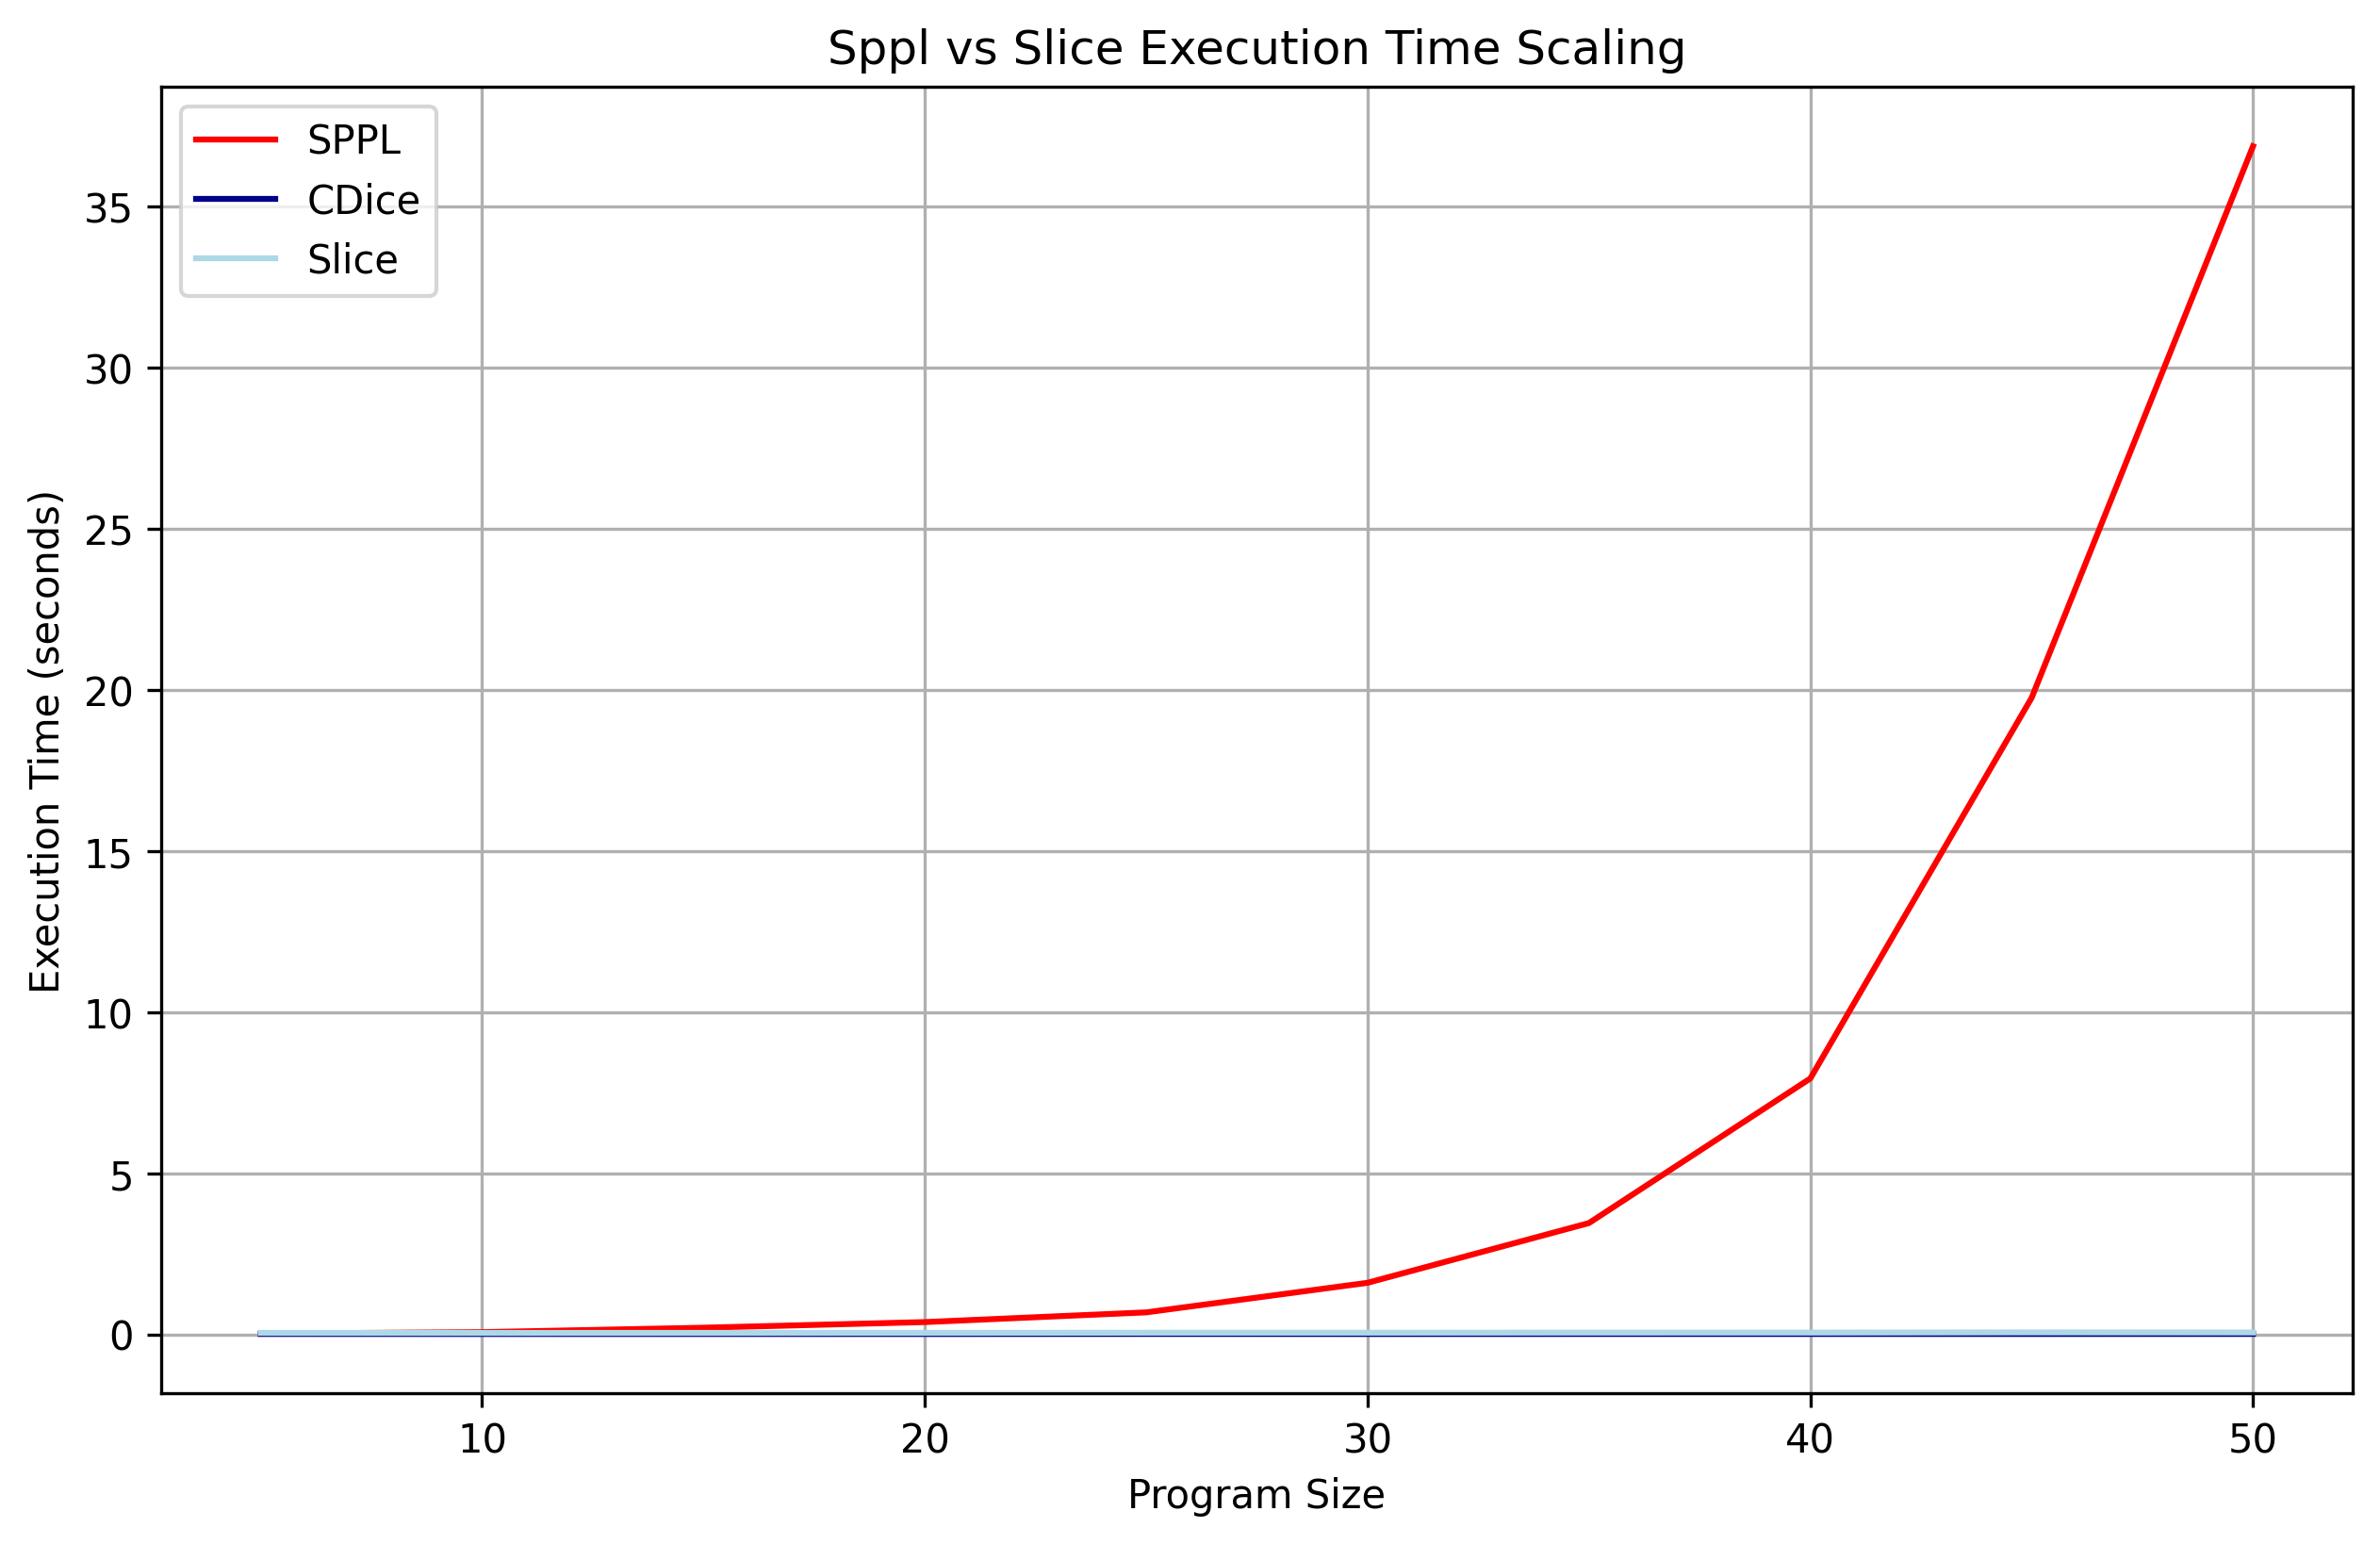
\includegraphics[width=\textwidth]{../images/scaling/build_alternating_guard_contdice_1.png}
\caption{Alternating Guard 1}
\label{fig:alt-benchmarks-a}
\end{subfigure}
\hfill
\begin{subfigure}{0.48\textwidth}
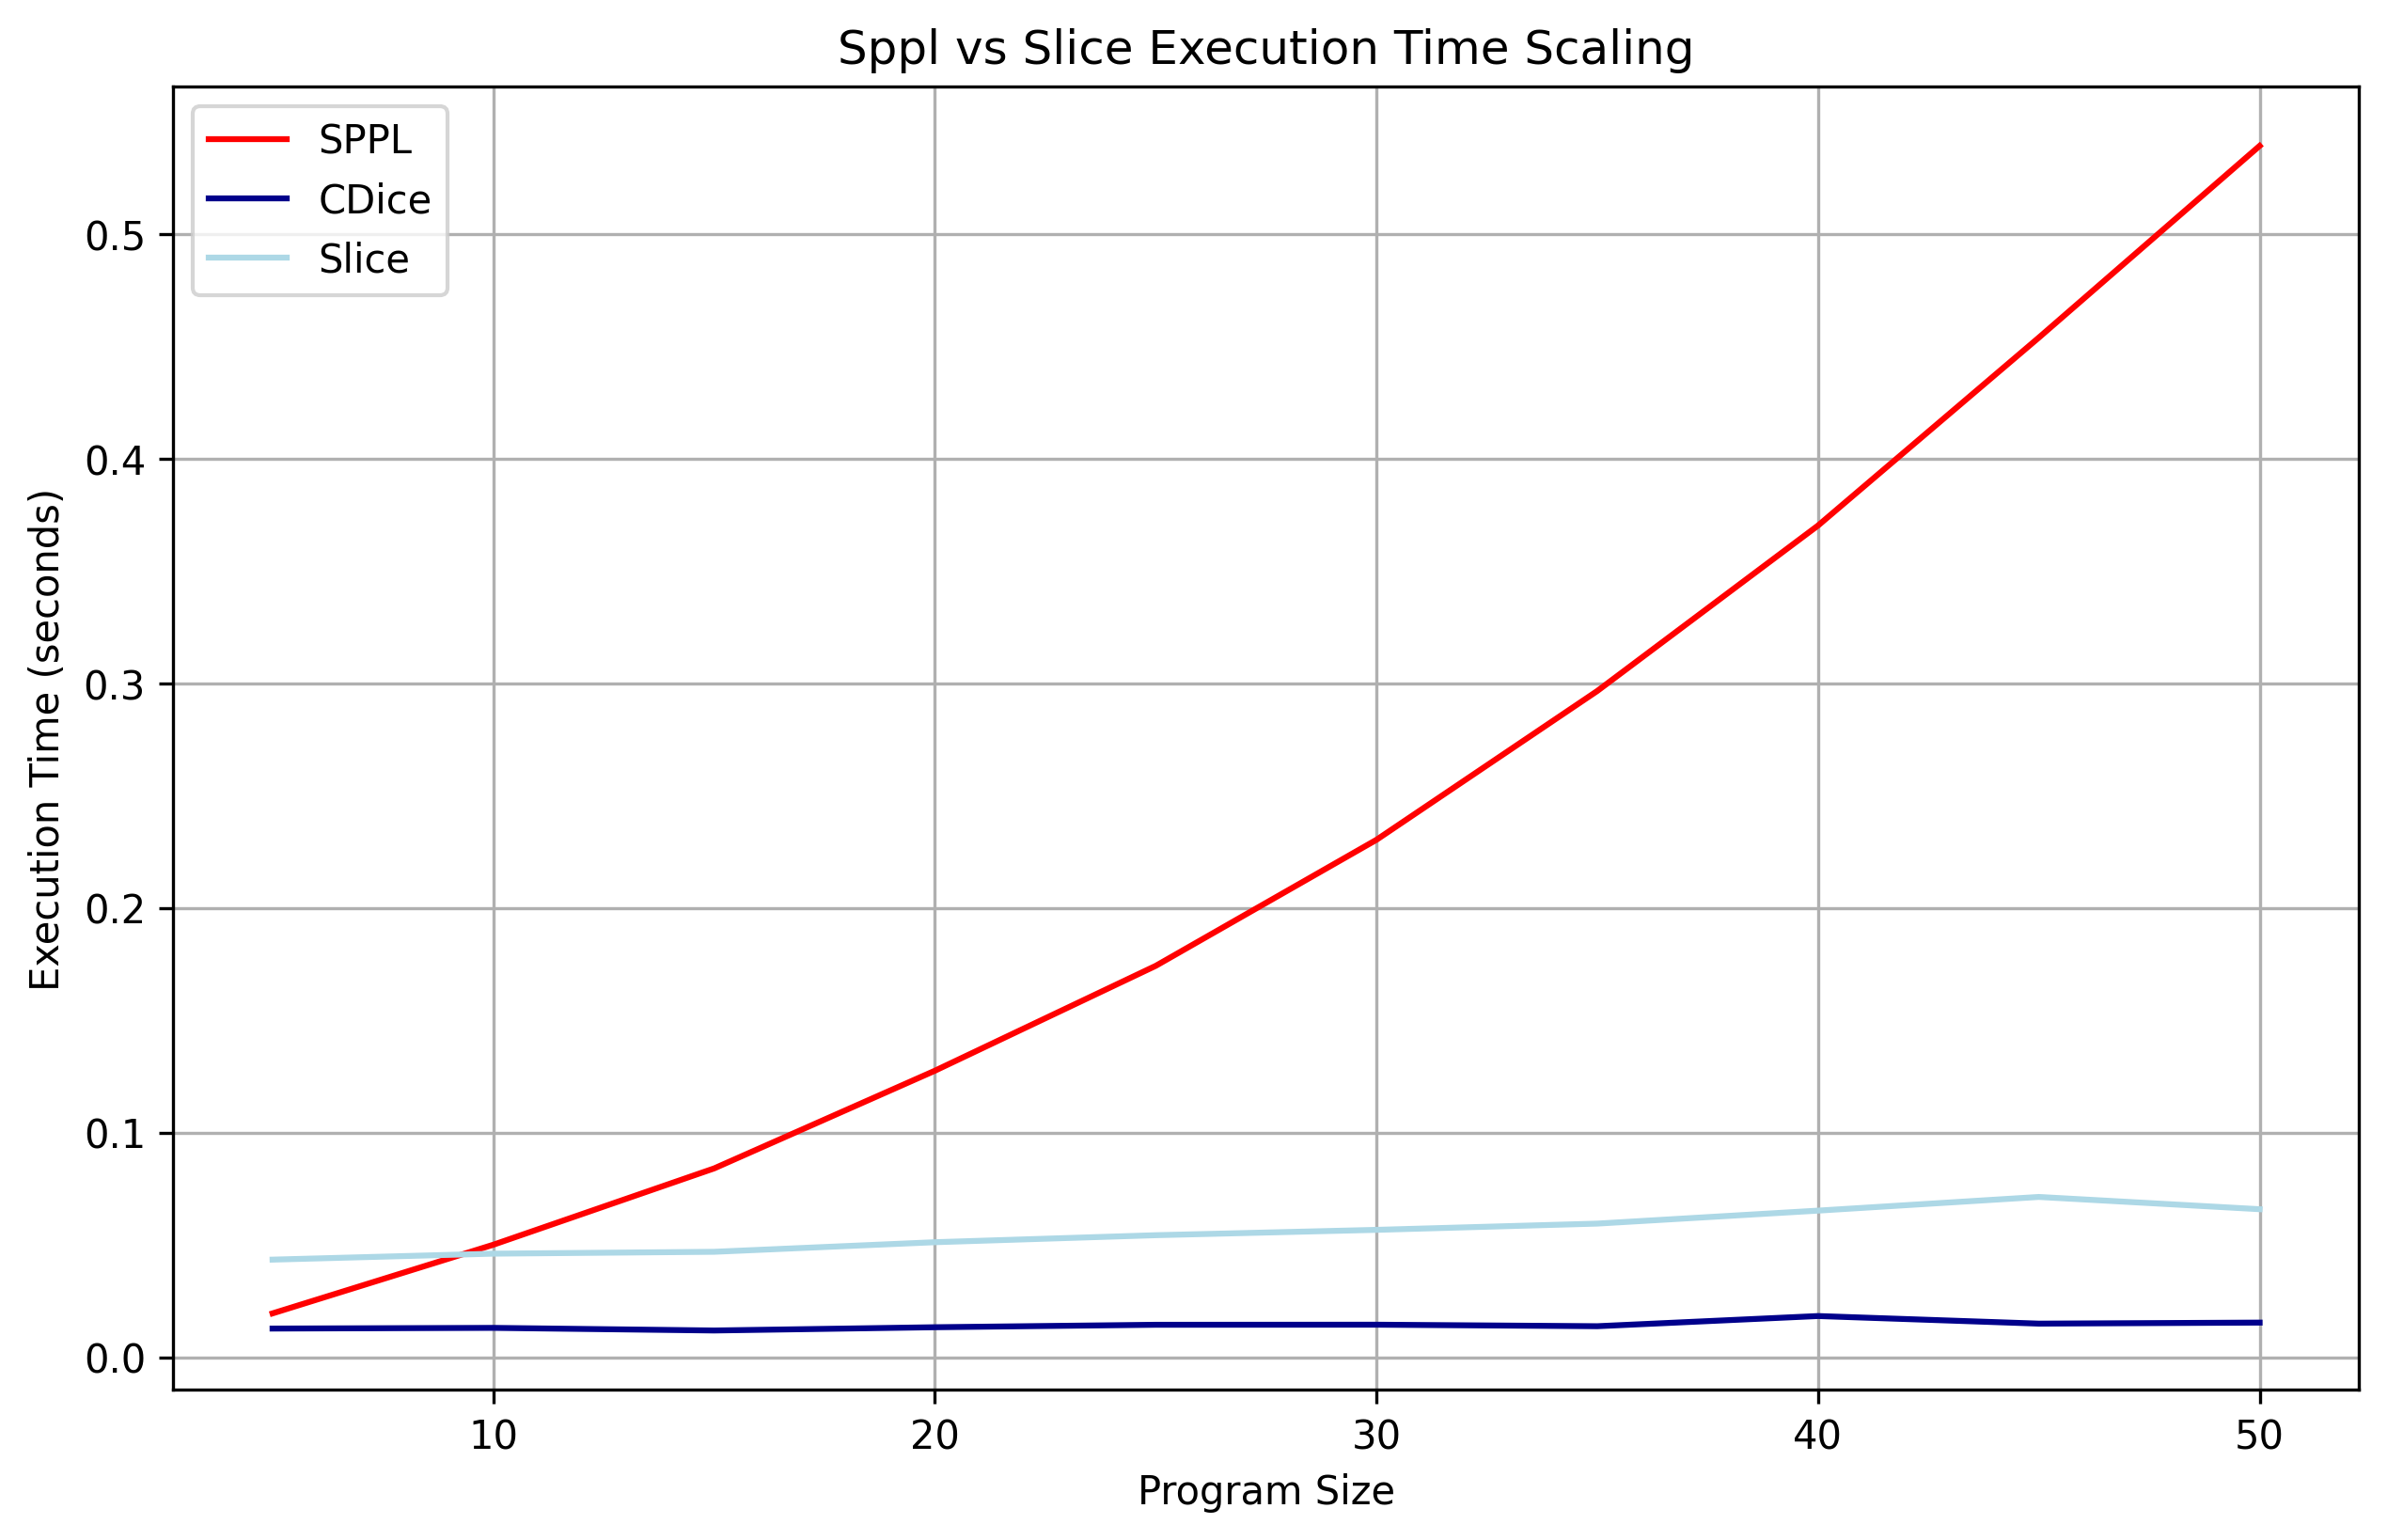
\includegraphics[width=\textwidth]{../images/scaling/build_alternating_guard_contdice_2.png}
\caption{Alternating Guard 2}
\label{fig:alt-benchmarks-b}
\end{subfigure}
\vspace{0.5em}
\begin{subfigure}{0.48\textwidth}
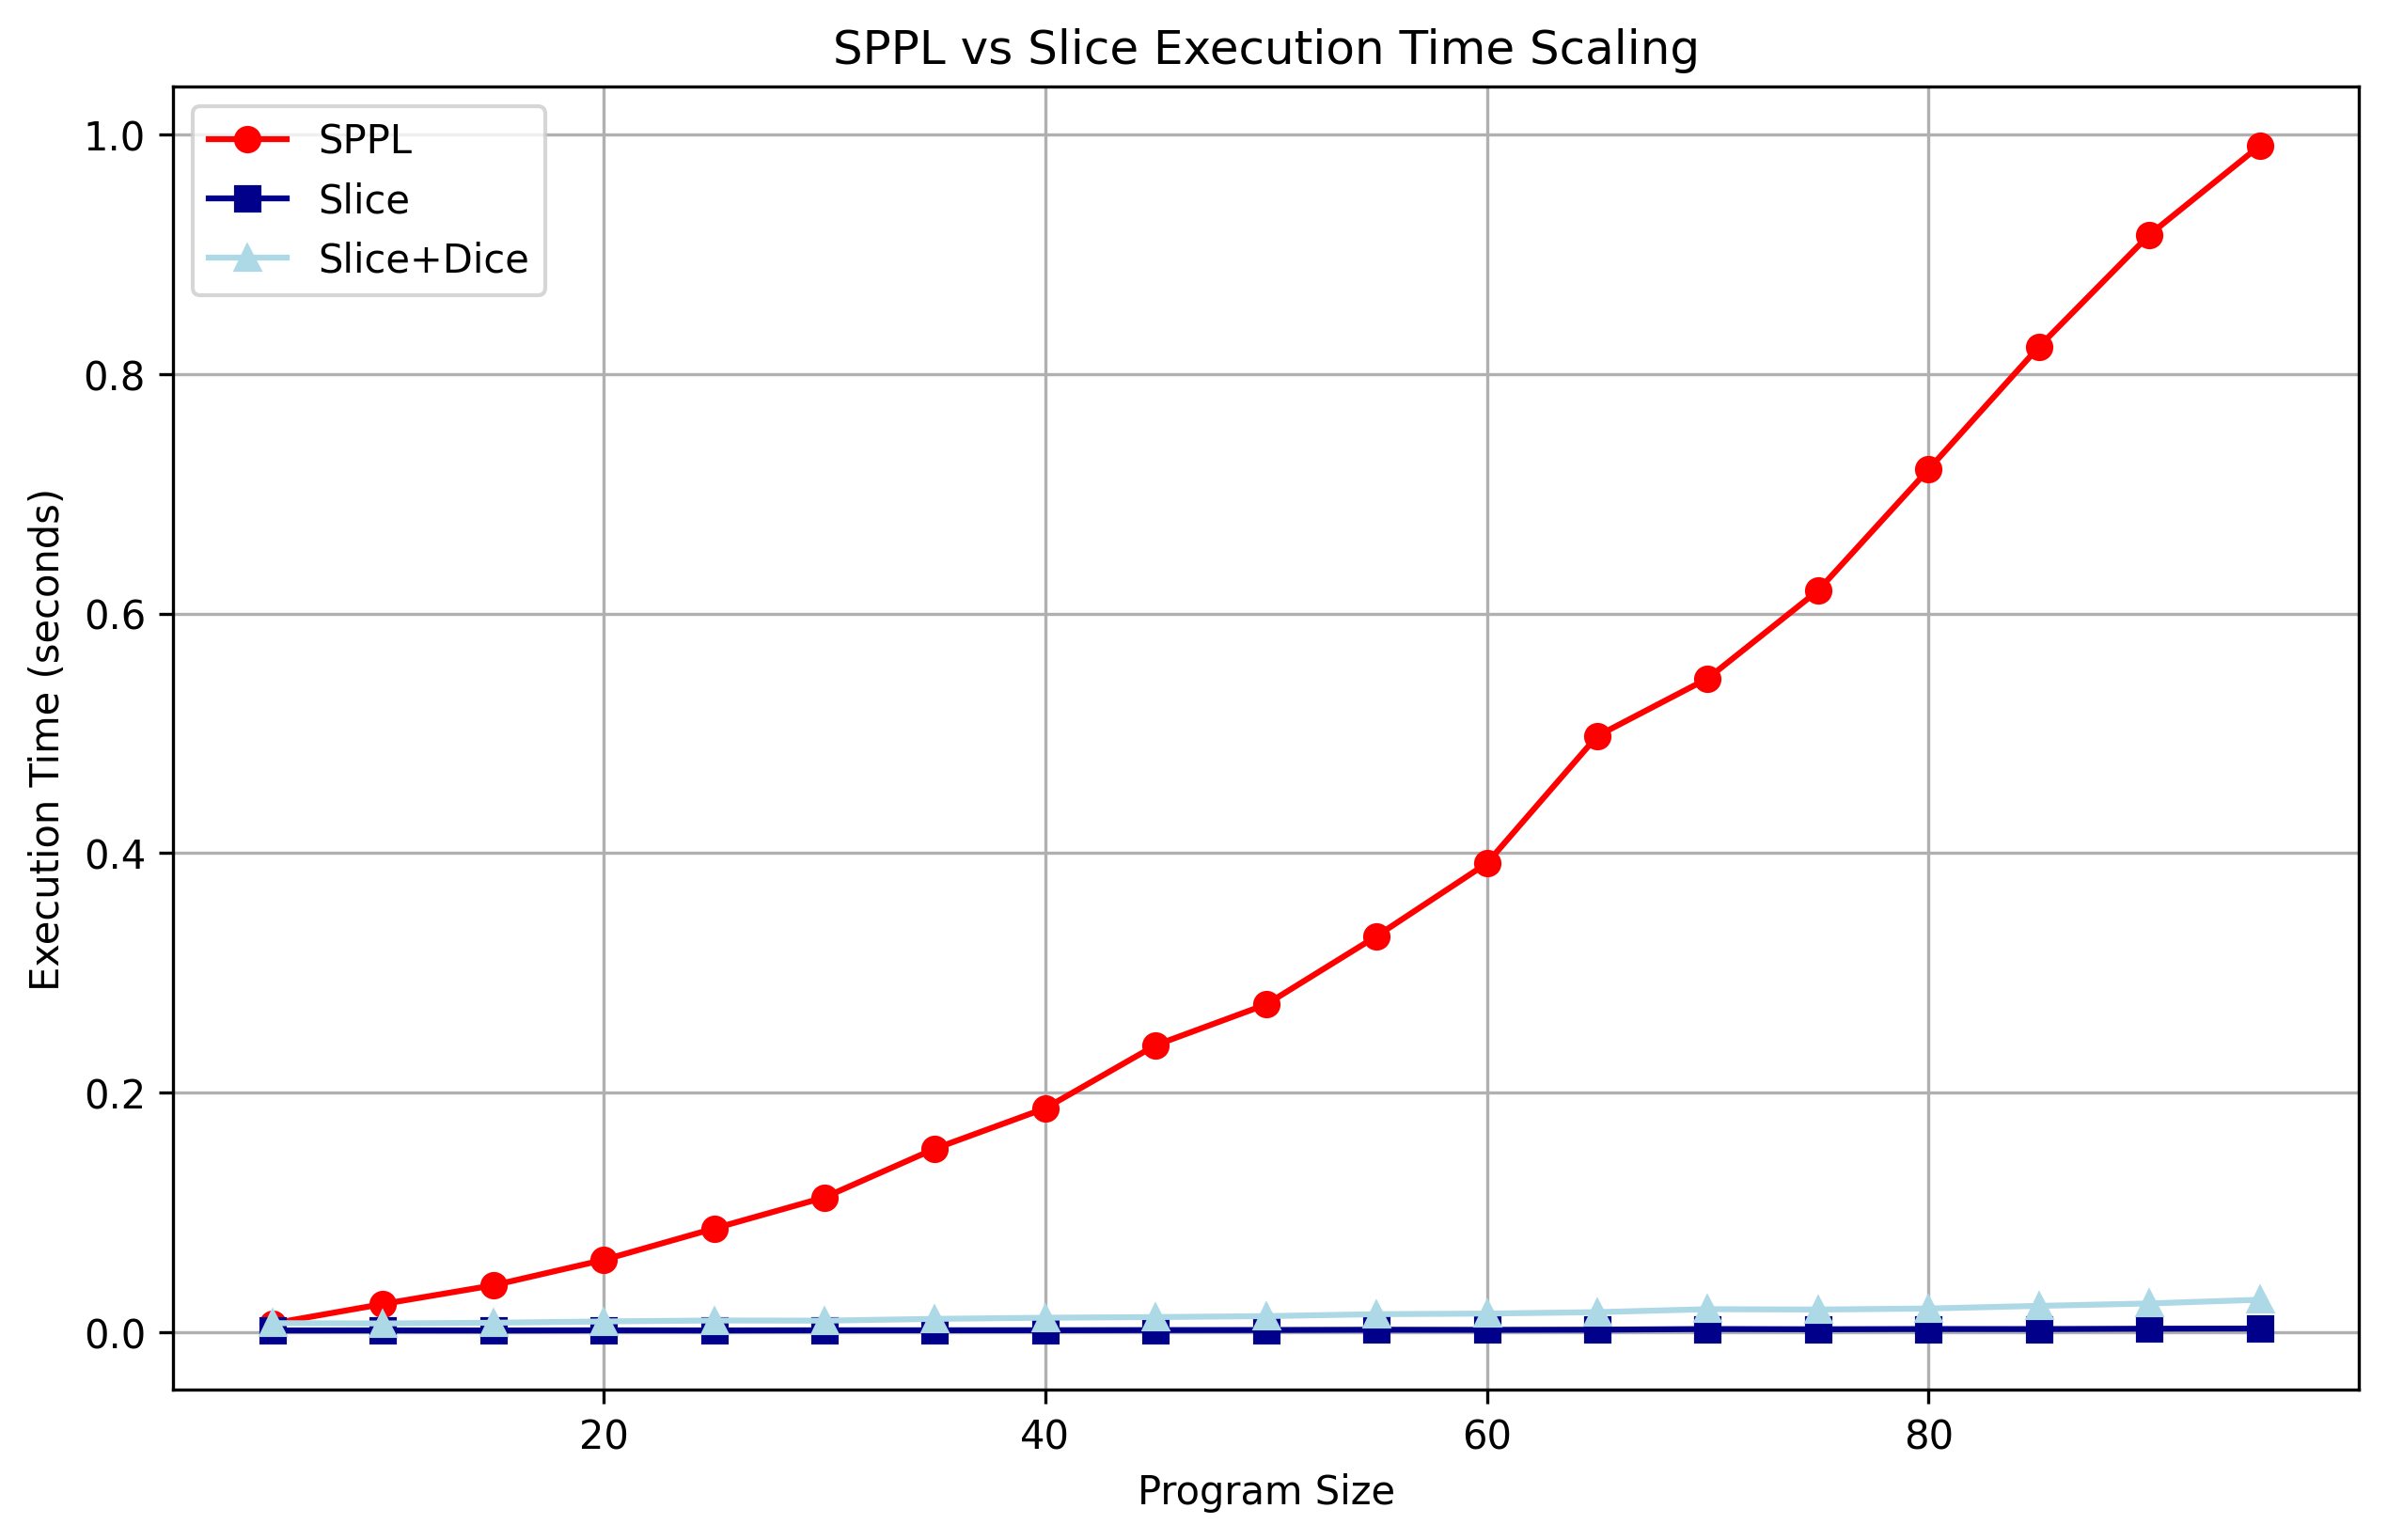
\includegraphics[width=\textwidth]{../images/scaling/build_alternating_guard_contdice_3.png}
\caption{Alternating Guard 3}
\label{fig:alt-benchmarks-c}
\end{subfigure}
\hfill
\begin{subfigure}{0.48\textwidth}
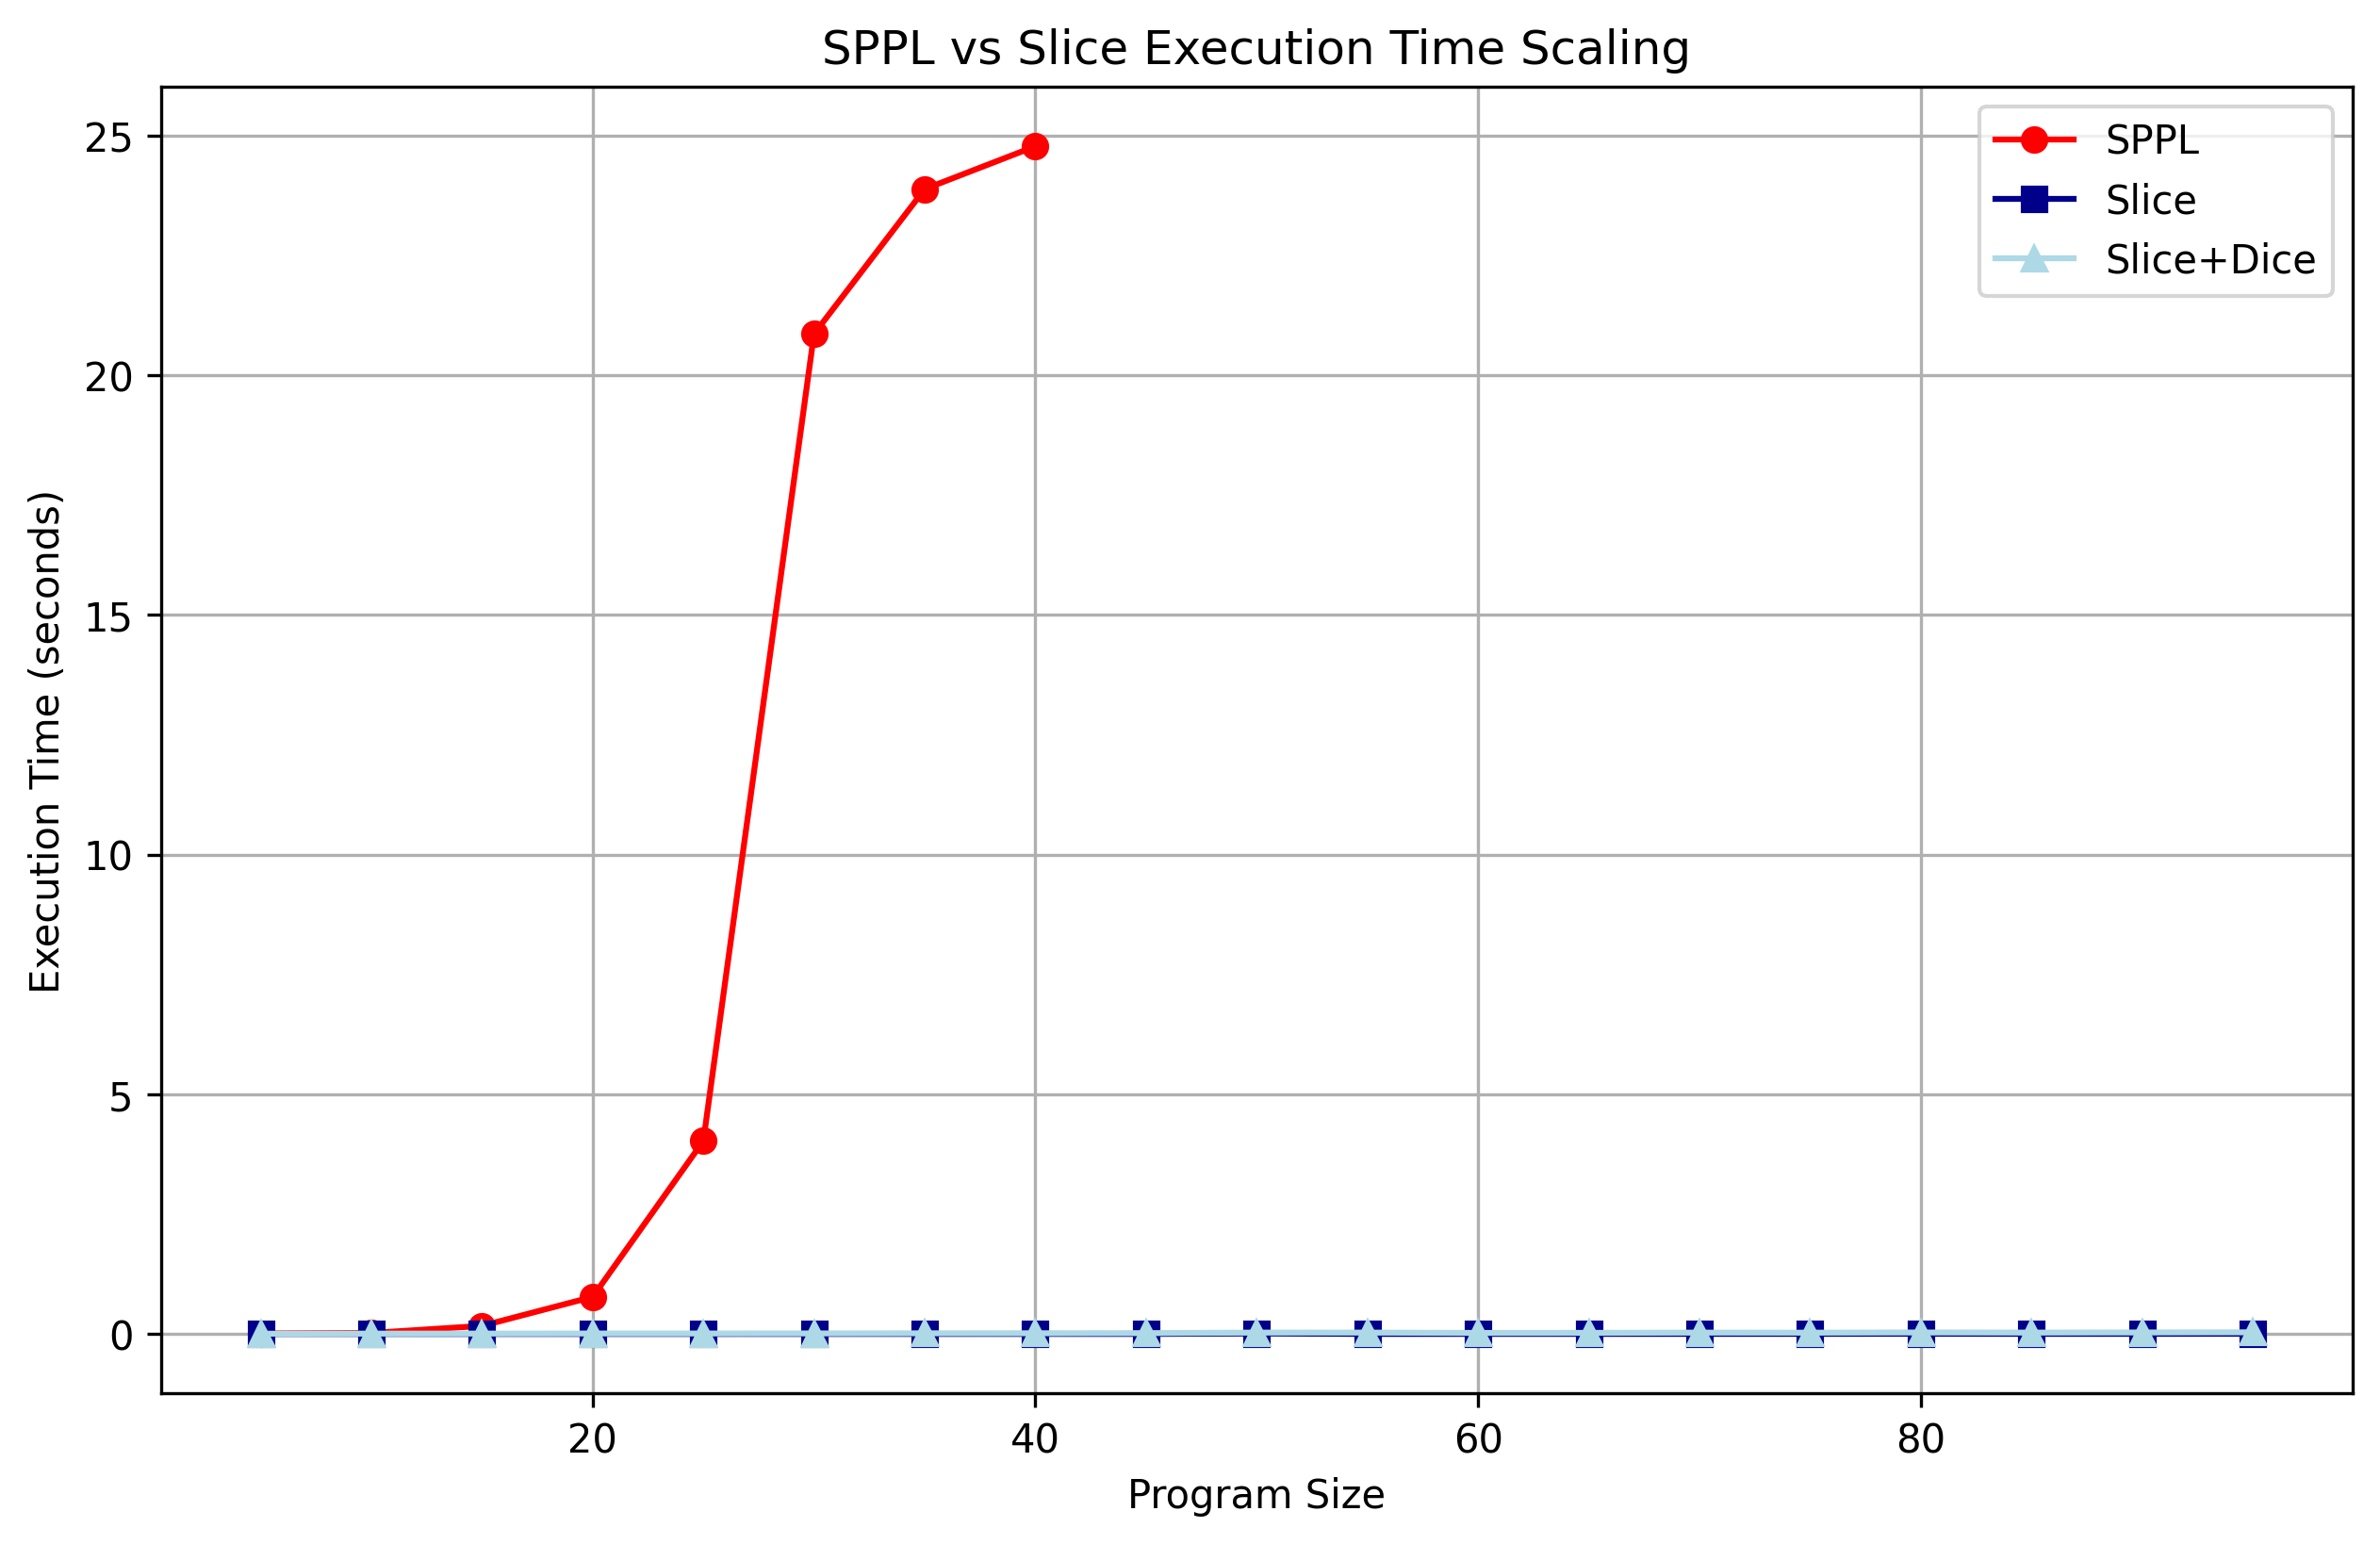
\includegraphics[width=\textwidth]{../images/scaling/build_random_alternating_guard_contdice.png}
\caption{Random Alternating Guard}
\label{fig:alt-benchmarks-d}
\end{subfigure}
\caption{Scaling results for alternating guard benchmarks. SPPL (red) times out early (between program sizes 20-30), while Slice continues to scale to large programs.}
\label{fig:alt-benchmarks}
\end{figure}

\paragraph{Results.} We generate programs of size 1-50 with step size 5 in each iteration for the conditional independence tests, and for the alternating guards tests, we generate programs of size 1-100 with step size 5 and 1 for the program size and guard span, respectively. We specify a timeout of 300s. The scaling experiments demonstrate that Slice maintains near-linear scaling behavior while SPPL exhibits significantly faster growth and times out on larger programs. Across all seven benchmarks, Slice+Dice execution time remains under 0.5 seconds even for programs with 90+ comparisons, while SPPL times out (at 300s) for programs as small as 20-30 in size. The Slice compilation phase alone (dark blue line) shows essentially constant time, indicating that the type-directed discretization algorithm scales extremely well.

\subsection{Fairness Benchmarks}
Characterizing the fairness of classification algorithms is an interesting application in machine learning. 


We evaluate Slice on decision tree models from the FairSquare suite with the following results:

\begin{table}[!t]
\centering
\begin{tabular}{lrrr}
\toprule
Benchmark & Slice+Dice (s) & SPPL (s) & Speedup \\
\midrule
DT4\_ind & 0.007 & 0.335 & 45.6× \\
DT4\_bn1 & 0.008 & 0.335 & 42.8× \\
DT4\_bn2 & 0.007 & 0.340 & 46.3× \\
DT14\_ind & 0.008 & 0.324 & 43.0× \\
DT14\_bn1 & 0.010 & 0.341 & 35.8× \\
DT14\_bn2 & 0.011 & 0.356 & 33.3× \\
DT16\_ind & 0.008 & 0.339 & 44.4× \\
DT16\_bn1 & 0.009 & 0.349 & 38.3× \\
DT16\_bn2 & 0.011 & 0.339 & 30.7× \\
DT44\_ind & 0.011 & 0.349 & 31.1× \\
DT44\_bn1 & 0.016 & 0.363 & 22.9× \\
DT44\_bn2 & 0.016 & 0.354 & 22.1× \\
\bottomrule
\end{tabular}
\caption{Execution times (seconds) for decision tree benchmarks}
\end{table}

\subsubsection{Clinical Trial Benchmark}
We evaluate Slice on a clinical trial model that uses discrete distributions to model treatment effectiveness:

\begin{table}[!t]
\centering
\begin{tabular}{lrrr}
\toprule
Benchmark & Slice+Dice (s) & SPPL (s) & Speedup \\
\midrule
Clinical Trial & 0.009 & 0.356 & 38.2× \\
\bottomrule
\end{tabular}
\caption{Execution times for clinical trial benchmark}
\end{table}


\subsection{Psi benchmarks}\label{sec:psi-benchmarks}
- describe benchmarks, cite paper
- simplications we made such as expanding out arrays
- graphs (slice + dice vs sppl vs bitblast)

\todo{Note: Psi benchmark files exist in dice/benchmarks/ but need to be ported to Slice syntax. Current .psi files include alarm, cancer, bayesian networks, etc.}

\subsection{Fairness benchmarks}\label{sec:fairness-benchmarks}
- describe benchmarks, cite paper
- simplications we made such as expanding out arrays
- graphs (slice + dice vs sppl vs bitblast)

\todo{Note: Fairness benchmarks need to be collected/created. The indian\_gpa example in examples/paper/ could be one fairness benchmark.}